%\part{Aspectos Gerais}

\chapter[Referencial Teórico]{Referencial Teórico}

\section{MEMS}

MEMS\footnote{Micro Electro Mechanical Systems - Sistema Micro-eletromecânicos}  é uma tecnologia de processamento usada para criar dispositivos integrados ou sistemas que combinam componentes mecânicos e elétricos. Eles são fabricado usando técnicas de processamento em lote de circuitos integrados e pode variar em tamanho entre alguns micrômetros para milímetros. Esses dispositivos (ou sistemas) têm a capacidade de detectar, controlar e atuar na escala micro e gerar efeitos em escala macro\cite{prime2002}. 

O termo MEMS, é um acrônimo originado nos Estados Unidos, também é conhecido como Microsystems Technology (MST) na Europa e Micromachines no Japão. Independentemente da terminologia, o fator de define um dispositivo MEMS está na maneira como é feito. Enquanto os aparelhos eletrônicos são fabricados usando tecnologia IC de 'chip de computador', os componentes micromecânicos são fabricados por sofisticadas manipulações com silício e outros substratos usando processos de micro-usinagem. Processos como micro-usinagem a granel e de superfície, bem como micromaquinação de alta proporção (HARM \footnote{high-aspect-ratio micromachining}) remove seletivamente partes do silício ou adiciona camadas estruturais adicionais para formar os componentes mecânicos e eletromecânicos. Enquanto circuitos integrados são projetados para explorar as propriedades elétricas do silício, o MEMS aproveita as propriedades mecânicas do silício ou suas propriedades elétricas e mecânicas\cite{prime2002}.

Na forma mais geral, os MEMS consistem em microestruturas mecânicas, microssensores, microatuadores e microeletrônica, todos integrados no mesmo chip de silício (Fig. \ref{esquematico_mems}). Microsensores detectam mudanças no ambiente do sistema medindo informações ou fenômenos mecânicos, térmicos, magnéticos, químicos ou eletromagnéticos. Microeletrônica processa essa informação e sinaliza aos microatuadores para reagirem e criarem alguma forma de mudanças no meio ambiente\cite{prime2002}.

\begin{figure}[h]
	\centering
	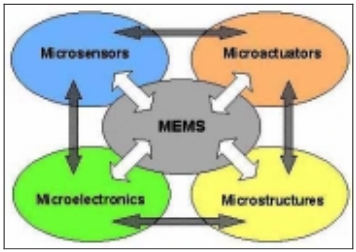
\includegraphics[keepaspectratio=true,scale=0.5
	]{figuras/esquematico_mems.png}
	\caption{Ilustração esquemática de componentes MEMS}
	Fonte: \cite{prime2002}
	\label{esquematico_mems}
\end{figure}

Os dispositivos MEMS são muito pequenos, seus componentes são geralmente microscópicos(Fig. \ref{escala_mems}). Alavancas, engrenagens, pistões, motores e até motores a vapor foram todos fabricados por MEMS. No entanto, MEMS não se refere apenas à miniaturização de componentes mecânicos ou à fabricação de coisas a partir do silício (na verdade, o termo MEMS é na verdade enganoso, já que muitos dispositivos micromachinados não são mecânicos em nenhum sentido). MEMS é uma tecnologia de fabricação; um paradigma para projetar e criar dispositivos e sistemas mecânicos complexos, bem como sua eletrônica integrada, utilizando técnicas de fabricação em lote\cite{prime2002}.

\begin{figure}[h]
	\centering
	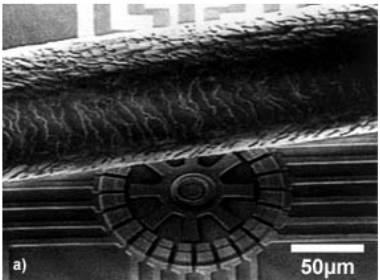
\includegraphics[keepaspectratio=true,scale=0.5
	]{figuras/escala_mems.png}
	\caption{Um motor MEMS ao lado de uma fio de cabelo humano.}
	Fonte: \cite{prime2002}
	\label{escala_mems}
\end{figure}

\section{IMU}

A história do sensor IMU começou em 1930, quando foi usado para auxiliar a navegação de aeronaves e outros dispositivos de grande porte. Por causa de suas restrições principalmente em tamanho, custo e consumo de energia, o uso da IMU naquele momento era restrito a aplicações em dispositivos grandes e, portanto, impopular para equipamentos de tamanho menor e em grande escala de consumo. Porém, recentemente, o sensor IMU feito por MEMS, foi introduzido com uma característica muito atraente de baixo custo, com poder de processamento e baixo custo. A demanda aumentou muito e as áreas de aplicação também. Atualmente, muitos fabricantes estão competindo nos melhores projetos de IMU, como Invensense, Honeywell, STMicroelectronics, Microstrain e X-Sens\cite{ahmad2013}.

Os sensores IMU podem ser capazes de medir diversas variáveis. Os mais comuns são feitos para medir 6 graus de liberdade. São 3 medidas de aceleração linear a partir de um acelerômetro e 3 medidas de aceleração angular feitas por um giroscópio (Fig.\ref{eixos_imu})\cite{santos2016}.
 
\begin{figure}[h]
	\centering
	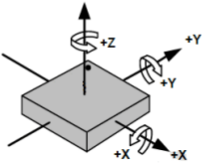
\includegraphics[keepaspectratio=true,scale=0.6
	]{figuras/Eixos_imu.png}
	\caption{Eixos de orientação.}
	Fonte adaptada de \cite{mpu6050}
	\label{eixos_imu}
	
\end{figure}


A vantagem de usar este tipo de IMU é que não será interferido pelo campo magnético externo em torno do
sensor quando é usado muito próximo de material ferromagnético. Por outro lado, dependendo do acelerômetro e do giroscópio, pode não ser suficiente para aumentar a precisão da medição devido ao ruído dos sensores e à questão do desvio do giroscópio. Os dados adquiridos pelo IMU são integrados como a mostrado na Figura \ref{integracao_imu} \cite{ahmad2013}.

\begin{figure}[h]
	\centering
	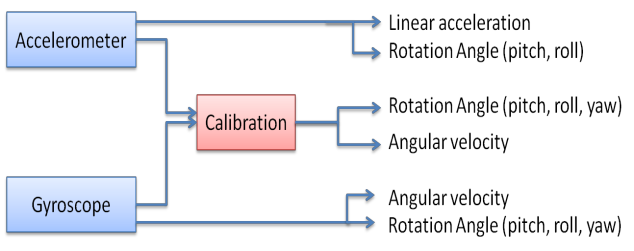
\includegraphics[keepaspectratio=true,scale=0.3
	]{figuras/integracao_imu.png}
	\caption{Sensor inercial baseado em 2 sensores}
	Fonte adaptada de \cite{ahmad2013}
	\label{integracao_imu}
	
\end{figure}

E com essas variáveis adquiridas um padrão de movimento pode ser traçado, e assim podem ser feitas análises sobre a movimentação humana. Assim, junto com a EMG\footnote{Eletromiografia}, o uso de sensores inercias tem sido mais solicitado na área de monitoramento de práticas esportivas\cite{howard2016}.

Porém, a utilização de IMU's com equipamentos de comunição sem fio, têm mostrado uma certa vantagem sobre o uso de sensores com EMG. Isso ocorre por conta de a integração entre acelerômetros, giroscópios e dispositivos de transmissão sem fio ser mais simplificada do que a aquisição de dados por eletromiógrafos sem fio\cite{howard2016}. 

Os testes que foram feitos com uso de sensores inerciais, segundo  Howard,2016 , foram capazes de produzir dados relaconados com fadiga muscular, perfomance, postura e velocidade. O que possibilita melhores técnicas de treinamento e até mesmo prevenção de lesão pode ser realizada.

\subsection{Acelerômetro}

O acelerômetro funciona a partir do efeito de cristais piezoelétricos, que é o princípio no qual alguns cristais geram uma corrente elétrica como resposta a uma pressão mecânica. Então o sensor acelerômetro  funciona como na Figura \ref{acel} demonstra, como uma pequena caixa com uma esfera dentro, e as paredes são os cristais piezoelétricos.  Sempre que a caixa é alterada de posição a esfera é forçada a se mover em direção de uma das paredes devido a força da gravidade ou de qualquer outra força de aceleração em outro sentido que não a normal. Cada par de paredes paralelos correspondem a um eixo no espaço. Assim, a partir da corrente gerada em cada parede é possível determinar a direção do movimento acelerado e sua magnitude\cite{sanjeev2018}.

\begin{figure}[h]
	\centering
	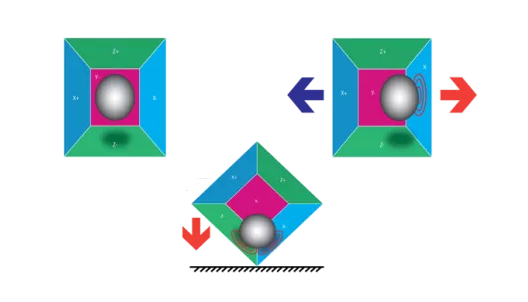
\includegraphics[keepaspectratio=true,scale=0.5
	]{figuras/acelerometro.png}
	\caption{Princípio de funcionamento do acelerômetro.}
	Fonte adaptada de NÃO SEI AINDA
	\label{acel}
	
\end{figure}

\subsection{Giroscópio}

\subsection{MPU6050}
	
	O MPU6050, é da séria MPU60X0, foi a primeira interface de movimento a integrar 6 eixos de leitura em um dispositivo único. Esse sensor de movimento, integra 3 eixos de um acelerômetro e 3 eixos de um gyroscópio e um DMP \footnote{\textit{Digital Motion Processor} - Processador Digital de Moviemento} tudo em um pequeno componente medindo 4x4x0.9mm. As suas principais qualidades são seu tamanho reduzido, o baixo consumo de energia, alta precisão e confiabilidade, alta tolerância a choques mecânicos, tem seu desempenho programável para aplicações específicas e ainda um baixo custo finaceiro. \cite{mpu6050}.
	
	O protocolo de comunicação utilizado pelo MPU6050 é o I2C\footnote{\textit{Inter-Integrated Circuit} - Circuito Inter-Integrado}. Que é um protocolo de barramento, e com os mesmos dois fios podem ser conectados vários dispositivos, um sendo o \textit{master} e os outros como \textit{slave}. Esta é uma característica boa para reduzir a quantidade de pinos necessários para conexão de mais dispositivos no microcontrolador.\cite{mpu6050}
	
	As aplicações, sugeridas pelo fabricante, para o MPU6050 são diversas, abaixo estão listadas algumas delas:
	\begin{itemize}
		\item Tecnologia \textit{ BlurFree\texttrademark }\footnote{Para estabilização de imagens e videos.}
		\item Controles para jogos baseados em movimento
		\item Sensores em roupas TouchAnywhere para aplicação na saúde e esportes
		\item Tecnologia \textit{ MotionCommand\texttrademark}\footnote{Para comandos de movimento curtos} 
		\item Em brinquedos
	\end{itemize}
	
	\begin{description}
		\item[Características do MPU6050] 
		\item \begin{itemize} 
			\item  O giroscópio, MEMS de 3 eixos do MPU6050, possui as seguintes características segundo \cite{mpu6050}:
			\begin{itemize}
				\item Saídas digitais com os valores de velocidade angular para os eixos X,Y e Z com escalas progrmáveis entre $ \pm250 $,$ \pm500 $,$ \pm1000 $ e $ \pm 2000$ deg/seg
				\item Conversores ADCs\footnote{Analog Digital Converter - Conversor Analógico Digital} de 16 bits integrados permitem amostragem simultânea do giroscópio
				\item Corrente de operação: 3.6mA
				\item Bom desempenho com ruído de baixa frequência
				\item Filtro passa-baixa programável.
				\item Fator de escala de sensibilidade calibrado de fábrica.
			\end{itemize}
			\item O acelerômetro, MEMS de 3 eixos do MPU6050, possui as seguintes características segundo \cite{mpu6050}:\begin{itemize}
				\item Saídas digitais dos 3 eixos do acelerômetro com escalas programáveis entre $\pm2g$, $\pm4g$, $\pm8g$ e $\pm16g$. Sendo \textquoteleft$ g$\textquoteright \ uma constante que equivale a aceleração da gravidade\footnote{aproximadamente $9,81 m/s^2 $}
				\item Conversores ADCs de 16 bits integrados permitem amostragem simultânea do acelerômetro sem a necessidade de um multiplexador
				\item Orientação, detecção e sinalização
				
			\end{itemize}
		\end{itemize}
	\end{description}
	
	
	

\subsection{Atmega328}

\section{Python}

\chapter[Metodologia]{Metodologia}

\section{Projeto de Hardware}

\section {Projeto de Software}

\chapter{Resultados e Discussão}

\chapter{Conclusão}